\documentclass[a4j]{jarticle}
\usepackage{graphicx}
\usepackage[left=25truemm,right=25truemm]{geometry}

\title{画像処理 レポート}

\author{氏名: 木下直樹\\学籍番号: 09425521}

\date{提出日: 2015月12月21日}

\begin{document}
\maketitle

%%%%%%%%%%%%%%%%%%%%%%%%%%%%%%%%%%%%%%%%%%%%%%%%%%
\section{MatrixLocalMaxの実装}
%%%%%%%%%%%%%%%%%%%%%%%%%%%%%%%%%%%%%%%%%%%%%%%%%%
ImageFeatureで得られる特徴点指標画像の極大値を探し, その座標を配列に記録するプログラムを実装する. 
得られた配列を降順にソートすることで適した任意の数の特徴点を扱うことができる. 
また, ソートアルゴリズムは挿入ソートを採用した. 

\begin{verbatim}
int MatrixLocalMax(int w[][2], Matrix*im2){
  int x,y,u,v,W=7,n=0,a;
  int i,j;
  int tmp[2],t;
   for(y=W+1;y<im2->H-W-1;y++) for(x=W+1;x<im2->W-W-1;x++){
       double max=-1;
       for(v=-W;v<=W;v++) for(u=-W;u<=W;u++){
	   // (x,y) を中心とする 15x15 の矩形領域内で DElem(im2,x+u,y+v) の最大値を探す.
	   if(max<DElem(im2,x+u,y+v)) max = DElem(im2,x+u,y+v);
	 }
       // 最大値が DElem(im2,x,y) と等しいなら,(x,y) を特徴点として記録する.
       if(max==DElem(im2,x,y)){
	 a=n++; w[a][0]=x; w[a][1]=y;
	 for(i=0;i<n;i++){
	   t=DElem(im2,w[i][0],w[i][1]);
	   tmp[0]=w[i][0]; tmp[1]=w[i][1];
	   for(j=i;j>=1 && DElem(im2,w[j-1][0],w[j-1][1])<t;j--){
	     w[j][0]=w[j-1][0]; w[j][1]=w[j-1][1];
	   }
	   w[j][0]=tmp[0]; w[j][1]=tmp[1];
	 }
       }
     }
   //for(i=0;i<n;i++)printf("%f\n",DElem(im2,w[i][0],w[i][1]));
   return n; // 記録した点の数
}
\end{verbatim}
上位30個の特徴点を出力した結果は以下である. 

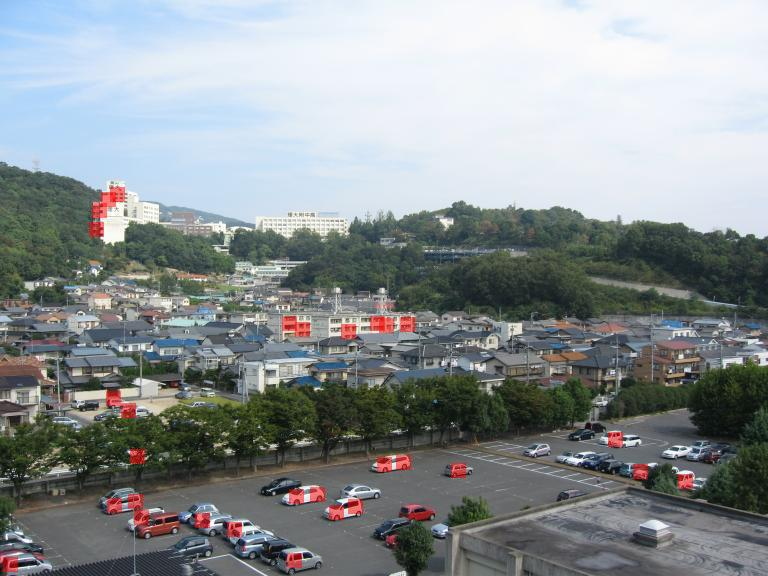
\includegraphics[bb=0 0 768 576,scale=.35]{out2.jpg}


\end{document}
